% !TEX options=--shell-escape
	\documentclass{article}
	\usepackage{amsmath,amssymb}
	\usepackage[inline]{enumitem}
	\usepackage{blindtext}
	\usepackage{booktabs}
	\usepackage{graphicx}
	\usepackage{xcolor}
	\usepackage[vmargin = 1.5in, top = 1in, bottom = 1.2in, letterpaper]{geometry}
	\usepackage{listings}
	\usepackage{courier}
	\usepackage{multicol}
	\usepackage{multirow}
	\usepackage{bm}
	\usepackage[labelformat=simple]{subcaption}
	\renewcommand\thesubfigure{(\alph{subfigure})}
	\usepackage{minted}
	\usepackage{fvextra}
	\definecolor{bg}{rgb}{0.95,0.95,0.95}
	\newminted{r}{mathescape, breaklines, linenos = true, bgcolor = bg}
	\usemintedstyle{tango}
	% \lstset{
	% basicstyle = \small\tt,
	% keywordstyle = \tt\color{blue},
	% commentstyle = \it\color[cmyk]{1,0,1,0},
	% stringstyle = \tt\color[RGB]{128,0,0},
	% %frame = single,
	% backgroundcolor = \color[RGB]{245,245,244},
	% breaklines,
	% extendedchars = false,
	% xleftmargin = 2em,
	% xrightmargin = 2em,
	% aboveskip = 1em,
	% tabsize = 4,
	% showspaces = false
	% }
	\newcommand\inner[2]{\left\langle{#1},{#2}\right\rangle}
	\DeclareMathOperator{\Corr}{Corr}
	\DeclareMathOperator{\Cov}{Cov}
	\DeclareMathOperator{\Var}{Var}
	\DeclareMathOperator{\E}{E}



	\begin{document}
	
	% \newfontfamily\courier{Courier New}

	
	\title{STAT 501 Homework 3}
	\author{Multinomial}
	\maketitle
	
	\begin{enumerate}[leftmargin = 0 em, label = \arabic*., font = \bfseries]
	\item 
	\begin{enumerate}
		\item 
		Let $\bm X = \begin{bmatrix}
					X_1& X_2& \ldots & X_n
				\end{bmatrix}^T$ and $\bm Y_1 = \begin{bmatrix}
					X_1 & X_2 & \ldots & X_{n-1}
				\end{bmatrix}^T,\, Y_2 = \bar{X}$. Since $X_1, \ldots ,X_n$ are iid $N(\mu, \sigma^2)$, then $\bm X \sim N_n(\bm \mu, \bm \Sigma)$, where $\bm \mu = \mu \bm 1_{n\times 1}$ and $\bm \Sigma = \sigma^2 \bm I_n$. We know
				\[\begin{bmatrix}
					\bm Y_1\\
					Y_2
				\end{bmatrix} = \begin{bmatrix}
					1 & 0 & \cdots & 0 & 0\\
					0 & 1 & \cdots & 0 & 0 \\
					\vdots & \vdots & \ddots & \vdots & \vdots\\
					0 & 0 & \cdots & 1 & 0\\
					\frac{1}{n} & \frac{1}{n} & \cdots & \frac{1}{n} & \frac{1}{n}
				\end{bmatrix} \bm X\]
				Hence $\begin{bmatrix}
					\bm Y_1 & Y_1
				\end{bmatrix}^T$ also follorws multivariate normal distribution. And we know 
				\[\E\left(\begin{bmatrix}
					\bm Y_1\\
					Y_2
				\end{bmatrix}\right) = \begin{bmatrix}
					\E\left(\begin{bmatrix}
											X_1 & \ldots & X_{n-1}
										\end{bmatrix}^T\right)&
					\E(\bar{X})
				\end{bmatrix}^T = \begin{bmatrix}
					\mu \bm 1_{(n-1)\times 1}\\
					\mu
				\end{bmatrix} = \begin{bmatrix}
					\bm \mu_1\\
					\bm \mu_2
				\end{bmatrix}\]

				\[\Var\left(\begin{bmatrix}
					\bm Y_1\\
					Y_2
				\end{bmatrix}\right) = \begin{bmatrix}
					\Var(\bm Y_1) & \Cov(\bm Y_1, Y_2)\\
					\Cov(Y_2, \bm Y_1^T) & \Var(Y_2)
				\end{bmatrix} = \begin{bmatrix}
					\sigma^2 \bm I_{n-1} & \frac{\sigma^2}{n} \bm 1_{(n - 1)\times 1}\\
					\frac{\sigma^2}{n} \bm 1_{1 \times (n-1)} & \frac{\sigma^2}{n} 
				\end{bmatrix} = \begin{bmatrix}
					\bm \Sigma_{11} & \bm \Sigma_{12}\\
					\bm \Sigma_{21} & \bm \Sigma_{22}
				\end{bmatrix}\]
				Thus we have
				\[\begin{bmatrix}
					\bm Y_1\\
					Y_2
				\end{bmatrix} \sim N_n \left(\begin{bmatrix}
					\bm \mu_1\\
					\bm \mu_2
				\end{bmatrix}, \begin{bmatrix}
					\bm \Sigma_{11} & \bm \Sigma_{12}\\
					\bm \Sigma_{21} & \bm \Sigma_{22}
				\end{bmatrix}\right).\]
				Thus we know
				\[\bm Y_1 | Y_2 \sim N_{n-1} (\bm \mu_{1} + \bm \Sigma_{12} \bm \Sigma_{22}^{-1} (Y_2 - \bm \mu_2), \bm \Sigma_{11} - \bm \Sigma_{12} \bm \Sigma_{22}^{-1} \bm \Sigma_{21})\]
				And
				\[\bm \mu_1 + \bm \Sigma_{12} \bm \Sigma_{22}^{-1} (Y_2 - \bm \mu_2) = \mu \bm 1_{(n-1)\times 1} + \frac{\sigma^2}{n} \bm 1_{(n-1)\times 1} \cdot \frac{n}{\sigma^2}(\bar{X} - \mu) = \bar{X} \bm 1_{(n-1)\times 1}\]
				\[\bm \Sigma_{11} - \bm \Sigma_{12} \bm \Sigma_{22}^{-1} \bm \Sigma_{21} = \sigma^2 \bm I_{n-1} - \frac{\sigma^2}{n} \bm 1_{(n-1)\times 1} \frac{n}{\sigma^2} \frac{\sigma^2}{n} \bm 1_{1 \times (n-1)} = \sigma^2 \bm I_{n-1} - \frac{\sigma^2}{n} \bm 1_{(n-1)\times (n-1)}\]
				Hence the distribution of $X_1, \ldots ,X_{n-1}$ given $\bar{X}$ is
				\[\begin{bmatrix}
					X_1 & \cdots & X_{n-1}
				\end{bmatrix}^T\big|\, \, \bar{X} \sim N_{n-1}\left( \bar{X} \bm 1_{(n-1)\times 1}, \sigma^2 \bm I_{n-1} - \frac{\sigma^2}{n} \bm 1_{(n-1)\times (n-1)}\right)\]
\newpage
				\item Function to generate $\bm X$ given $\bar{X}$.
				\begin{rcode}
# 1(b) generate random vector X given X-bar.
library(MASS)
X.gen <- function(xbar, n, sigma){
  mu <- rep(xbar, n-1)
  Sigma <- diag(rep(sigma^2, n-1)) - matrix(rep((sigma^2/n), (n-1)*(n-1)), nrow = n-1)
  Y1 <- mvrnorm(mu = mu, Sigma = Sigma)
  X <- c(Y1, n*xbar - sum(Y1))
  return(X)
}
				\end{rcode}

				\item The R code to obtain a higher resolution image is shown below.
				\begin{rcode}
# 1(c) 
## i. & iii.
## read the image
library(rtiff)
owlet <- readTiff(fn = "Indian_spotted_owlet.tiff")
plot(owlet)



## function super resolution one pixel to 4x4, and truncate at 0 and 1
supres <- function(x){
  y <- X.gen(x, 16, 0.4)
  y1 <- ifelse(y < 0, 0, y)
  y2 <- ifelse(y1 > 1, 1, y1)
  return(matrix(y2, nrow = 4))
}

## high resolution matrix for red channel
size.low <- owlet@size
owletsupr <- apply(X = owlet@red, MARGIN = c(1,2), FUN = supres)
owletsupr1 <- array(dim = c(4,4)*size.low)
for(i in 1:size.low[1]){
  for(j in 1:size.low[2]){
    for(k in 1:4){
      for(l in 1:4){
        owletsupr1[4*(i - 1) + k, 4*(j-1) + l] <- owletsupr[4*(k-1) + l, i, j]
      }
    }
  }
}

## ii.
## high resolution matrix for green and blue

### green channel
owletsupg <- apply(X = owlet@green, MARGIN = c(1,2), FUN = supres)
owletsupg1 <- array(dim = c(4,4)*size.low)
for(i in 1:size.low[1]){
  for(j in 1:size.low[2]){
    for(k in 1:4){
      for(l in 1:4){
        owletsupg1[4*(i - 1) + k, 4*(j-1) + l] <- owletsupg[4*(k-1) + l, i, j]
      }
    }
  }
}

### blue channel
owletsupb <- apply(X = owlet@blue, MARGIN = c(1,2), FUN = supres)
owletsupb1 <- array(dim = c(4,4)*size.low)
for(i in 1:size.low[1]){
  for(j in 1:size.low[2]){
    for(k in 1:4){
      for(l in 1:4){
        owletsupb1[4*(i - 1) + k, 4*(j-1) + l] <- owletsupb[4*(k-1) + l, i, j]
      }
    }
  }
}



owlet.high <- array(dim  = c(owlet@size*c(4,4), 3))
owlet.high[,,1] <- owletsupr1
owlet.high[,,2] <- owletsupg1
owlet.high[,,3] <- owletsupb1

## iv.
### create pixmap object
owlet.highres <- pixmapRGB(owlet.high)

## v.
### display the high resolution image, save
par(mar=c(0,0,0,0))
plot(owlet.highres)
writeTiff(owlet.highres, fn = "./owlet_high.tiff")
				\end{rcode}
				\newpage
				And the higher resolution image is as below in Figure~\ref{high}. We can see there is more noise compared to the original one in Figure~\ref{low}.
				\begin{figure}[!htb]
				\centering
				\includegraphics[width = 0.7\textwidth]{high_res.jpeg}
				\caption{Higher resolution image}
				\label{high}
				\end{figure}

				\begin{figure}[!htb]
				\centering
				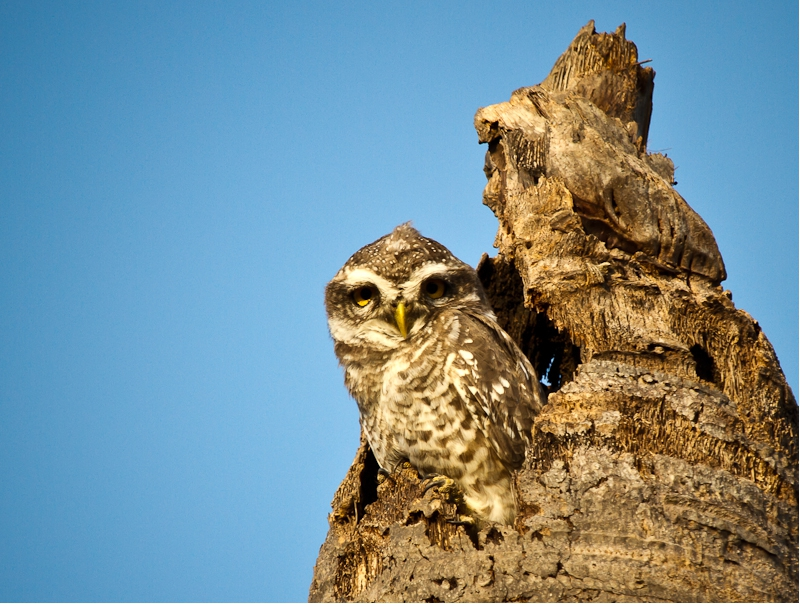
\includegraphics[width = 0.7\textwidth]{original.jpeg}
				\caption{Original image}
				\label{low}
				\end{figure}


	\end{enumerate}
	\newpage

	\item 
	\begin{enumerate}
		\item 
		When $\theta = 0$, $Y_i = g(X_i, 0) = X_i \sim N(\mu_0, \sigma_0^2)$. So the cdf of $\bm X_i$ is
		\[f(x) = \frac{1}{\sqrt{2 \pi} \sigma_0} \exp\left(-\frac{(x - \mu_0)^2}{2 \sigma_0^2}\right)\]
		when $\theta > 0$, then
		\[f(x) = f_{Y}(g(x, \theta))\left|\frac{\partial g}{\partial x}\right| = \frac{1}{\sqrt{2 \pi} \sigma_{\theta}} \exp\left(-\frac{(\mathrm{arcsinh}(\theta x)/\theta - \mu_{\theta} )^2}{2 \sigma_\theta^2}\right) \frac{1}{\sqrt{1 + \theta^2 x^2}}\]
		So in summary,
		\[f(x) = \frac{1}{\sqrt{2 \pi} \sigma_{\theta}} \exp\left(-\frac{(g(x, \theta) - \mu_{\theta} )^2}{2 \sigma_\theta^2}\right) \frac{1}{\sqrt{1 + \theta^2 x^2}},\, \theta \geq 0\]
		Thus the log likelihood is
		\[\ell(\theta, \mu_\theta, \sigma_\theta^2) = \sum_{i=1}^n \log f(x_i) = -\frac{n}{2} \log 2 \pi - n \log \sigma_\theta - \frac{1}{2 \sigma_\theta^2} \sum_{i=1}^n \left(g(x_i, \theta) - \mu_\theta\right)^2 - \frac{1}{2} \sum_{i=1}^n \log(1 + \theta^2 x_i^2), \, \theta \ge 0\]

		And we also know for a fixed $\theta$, 
		\begin{align*}
		& \hat{\mu}_\theta = \frac{\sum_{i=1}^n g(x_i, \theta)}{n}\\
		& \hat{\sigma}_\theta^2 = \frac{\sum_{i=1}^n \left(g(x_i, \theta) - \hat{\mu}_\theta\right)^2}{n}
		\end{align*}
		Then the maximized log likelihood for a fixed $\theta$ is
		\begin{align*}
		\hat{\ell}(\theta) &=  - \frac{n}{2} \log ( 2 \pi \hat{\sigma}_\theta^2) - \frac{1}{2 \hat{\sigma}_\theta^2} \sum_{i=1}^n \left(g(x_i, \theta) - \hat{\mu}_\theta\right)^2 - \frac{1}{2} \sum_{i=1}^n \log(1 + \theta^2 x_i^2)\\
		& = -\frac{n}{2} \log(2 \pi \hat{\sigma}_\theta^2) - \frac{n}{2} - \frac{1}{2} \sum_{i=1}^n \log(1 + \theta^2 x_i^2),\, \theta \geq 0
		\end{align*}
		\item 
	\begin{enumerate}
		\item 
		We first look at the summary and histogram of \verb|danish|.
		\begin{rcode}
# 2.
## 2 (b) i.
library(SMPracticals)
summary(danish)
hist(danish)
		\end{rcode}
		Then we have the summary
		\begin{rcode}
    Min.  1st Qu.   Median     Mean  3rd Qu.     Max. 
  0.3134   1.1572   1.6339   3.0627   2.6455 263.2504 
		\end{rcode}
		\newpage
		and the histogram as in Figure~\ref{danish_hist}.
		\begin{figure}[!htb]
			\centering
			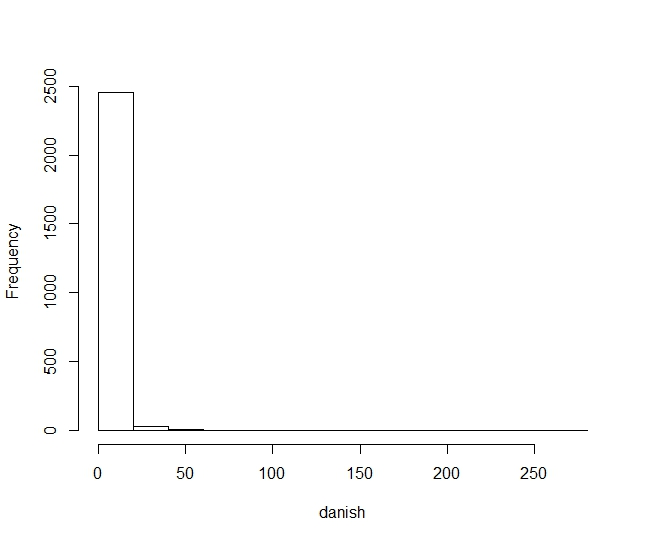
\includegraphics[width = 0.5\textwidth]{danish_hist.jpeg}
			\caption{Histogram of \texttt{danish}}
			\label{danish_hist}
		\end{figure}
		We can see from the histogram and the summary a lot of mass is close to 0 (and less than 3).

		Then we removed the potential outliers and make the histogram again.
		\begin{rcode}
## remove the potential outlier
danish1 <- danish[!danish %in% boxplot.stats(danish)$out]
hist(danish1)
		\end{rcode}
		The histogram is shown in Figure~\ref{danish1_hist}.
		\begin{figure}[!htb]
			\centering
			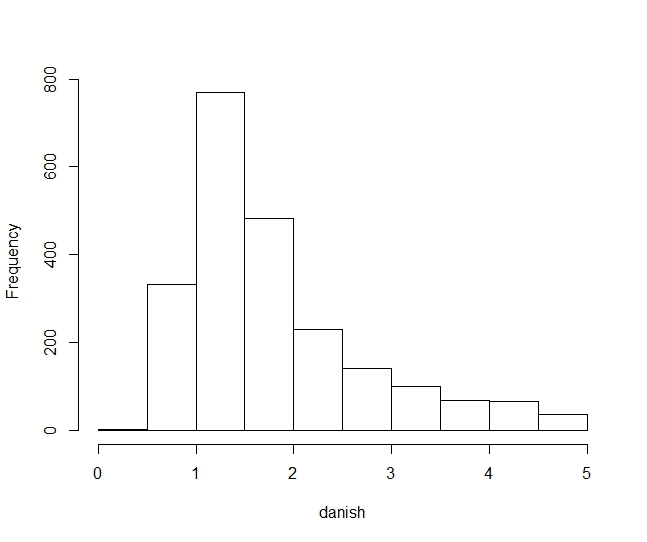
\includegraphics[width = 0.5\textwidth]{danish1_hist.jpeg}
			\caption{Histogram of \texttt{danish} with potential outliers removed}
			\label{danish1_hist}
		\end{figure}

		Here we can see the distribution is right skewed and the center is around 1.5. A lot of mass is between 1 and 2.

\newpage
	\item 
	By varying $\theta$ in $[0,4]$ with step size 0.1, we can obtain the curve of maximized log likelihood against $\theta$. The R codes for the curve are shown below.
	\begin{rcode}
## 2 (b) ii.
### define g function
g <- function(x, theta){
  if(theta == 0)
    return(x)
  else
    return(asinh(theta*x)/theta)
}

### define the maximized log likelihood
ell <- function(x, theta){
  n <- length(x)
  y <- g(x, theta)
  muhat <- sum(y)/n
  sigmahat2 <- sum((y - muhat)^2)/n
  return(-(n/2)*log(2*pi* sigmahat2) - (n/2) - sum(log(1 + theta^2 * x^2))/2)
}

### find maxmized log likelihood for each theta and plot the curve
thetas <- seq(0, 4, 0.1)
ells <- sapply(thetas, ell, x = danish)
plot(x = thetas, y = ells, 'n',xlab = "theta", ylab = "maximized logLik")
lines(x = thetas, y = ells)

### plot between theta from 3 to 4
thetas1 <- thetas[thetas >= 3]
ells1 <- ells[thetas >= 3]
plot(x = thetas1, y = ells1, 'n',xlab = "theta", ylab = "maximized logLik")
lines(x = thetas1, y = ells1)
	 \end{rcode} 

	 In Figure~\ref{ltheta04}, we can see the curve is increasing and becoming flat after 3. Then we plot the curve for $\theta \in [3,4]$ in Figure~\ref{ltheta34} to have a better idea of the trend. Hence the maximized log likelihood for $\theta \in [0,4]$ attains the maximum when $\theta = 4$.  
	 \begin{figure}[!htb]
	     \centering
	 	\begin{subfigure}[b]{0.4\textwidth}
	 	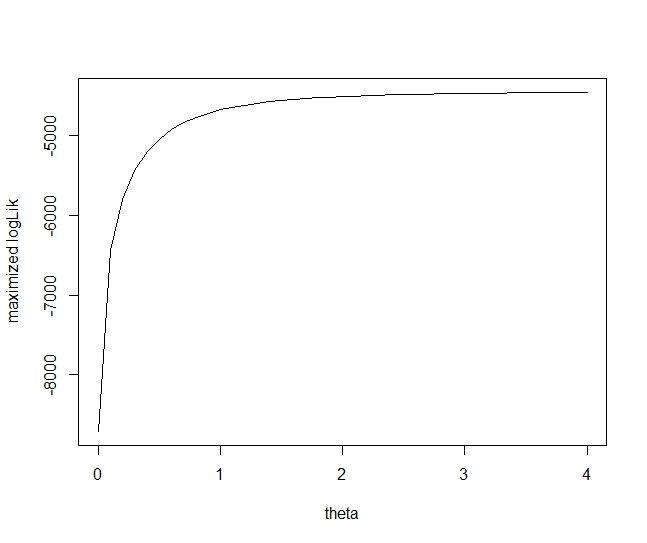
\includegraphics[width = \textwidth]{ltheta04.jpeg}
	 	\caption{$\hat{\ell}(\theta)$ for $\theta \in [0,4]$}
	 	\label{ltheta04}
	 	\end{subfigure}%
	 	\begin{subfigure}[b]{0.4\textwidth}
	 	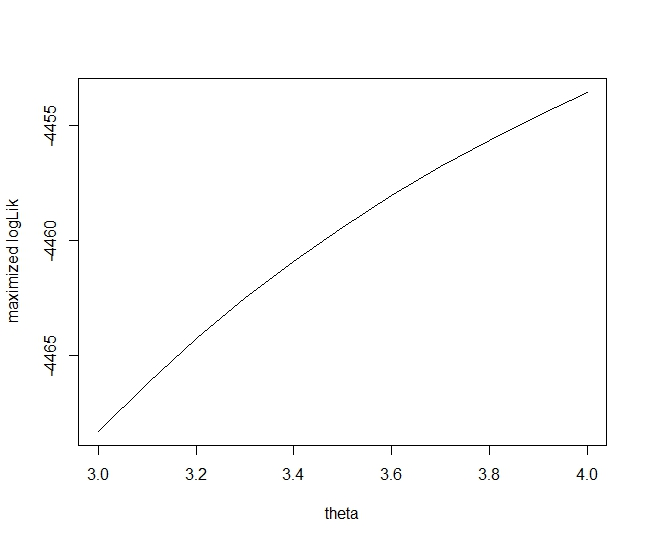
\includegraphics[width = \textwidth]{ltheta34.jpeg}
	 	\caption{$\hat{\ell}(\theta)$ for $\theta \in [3,4]$}
	 	\label{ltheta34}
	 	\end{subfigure}
	    \caption{Maximized log likelihood $\hat{\ell}(\theta)$ against $\theta$}
	 \end{figure}
	\newpage
Thus we use $g(x, 4)$ to transform \verb|danish|. And we plot the histogram in Figure~\ref{histg} and Q-Q plot of transformed data in Figure~\ref{qq}. 

\begin{rcode}
### transform the data with theta = 4
transformed_danish <- g(danish, 4)

hist(transformed_danish, main = "")

qqnorm(transformed_danish, main = "")
\end{rcode}

\begin{figure}[!htb]
     \centering
 	\begin{subfigure}[b]{0.4\textwidth}
 	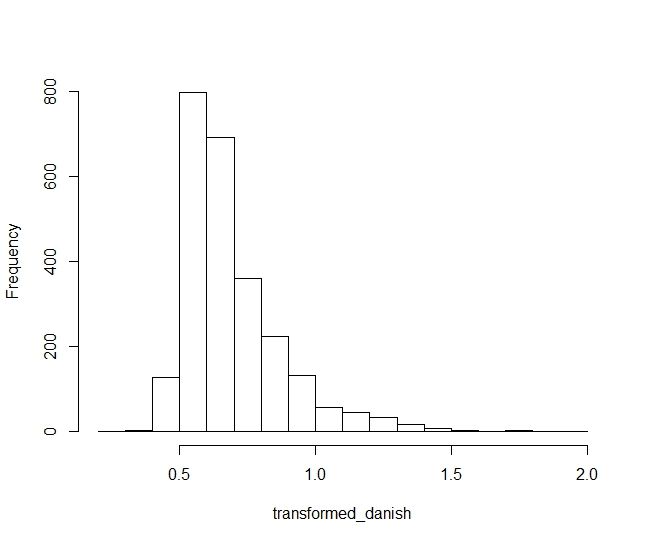
\includegraphics[width = \textwidth]{histg.jpeg}
 	\caption{Histogram of transformed \texttt{danish}}
 	\label{histg}
 	\end{subfigure}%
 	\begin{subfigure}[b]{0.4\textwidth}
 	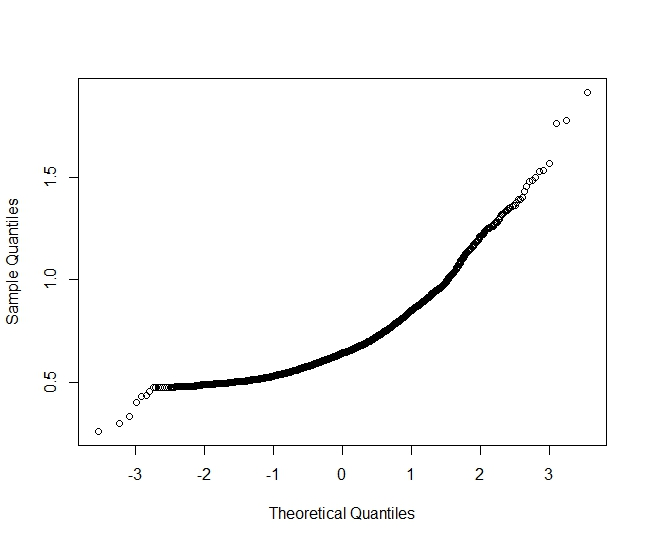
\includegraphics[width = \textwidth]{qq.jpeg}
 	\caption{Q-Q plot of transform \texttt{danish}}
 	\label{qq}
 	\end{subfigure}
 	\caption{Graphical display of transformed \texttt{danish}}
 \end{figure} 

 We can see the histogram is not quite symmetric and the Q-Q plot is apparently a curve, not a straight line. So the transformed data is not likely to be normally distributed.
\newpage
We then did a Shapiro-Wilk's test, and the p-value is small, thus the transformed data are not normal.
\begin{rcode}
### shapiro-wilk's test
shapiro.test(transformed_danish)
\end{rcode}
The result is
\begin{rcode}
	Shapiro-Wilk normality test

data:  transformed_danish
W = 0.85989, p-value < 2.2e-16
\end{rcode}
	\end{enumerate}

	\end{enumerate}


	
	
		\end{enumerate}










	
	
	
	\end{document}